\documentclass[a4paper,10pt,oneside]{article}
\usepackage[polutonikogreek,italian]{babel}
\usepackage[utf8x]{inputenc}
\usepackage{amsmath}
\usepackage{amsthm}
\usepackage{amssymb}
\usepackage{amscd}
\usepackage{graphicx}
\usepackage{float}
\usepackage{array}
\usepackage{rotating}
\usepackage[small]{caption}
\usepackage{lscape}
\usepackage{fancybox}
\usepackage{booktabs}
\usepackage[noanswer]{exercise}
\parindent0ex
\renewcommand{\fboxsep}{0.4cm}
\usepackage{hyperref}
\renewcommand{\textfraction}{0.05}
\renewcommand{\topfraction}{0.95}
\renewcommand{\bottomfraction}{0.95}
\renewcommand{\floatpagefraction}{0.35}
\renewcommand{\ExerciseName}{Esercizio}
\renewcommand{\ExerciseListName}{Es}
\setcounter{totalnumber}{5}
\restylefloat{figure}
\begin{document}

\section*{Energia potenziale  e oscillatori armonici}

\vspace{1cm}

Definiamo  l'energia potenziale di un  campo di forze \emph{conservative} dicendo che la sua variazione da un punto $A$ ad un punto $B$ dello spazio è pari al lavoro fatto \textbf{contro} le forze del campo per spostare una massa $m$ dal punto $A$ al punto $B$.
Definiamo la forza applicata:
\begin{equation}
 \mathbf{F}_{app}=-\mathbf{F}_c
\end{equation}
dove $\mathbf{F}_{app}$ è la forza che esercitiamo per spostare l'oggetto all'interno del campo di forze $\mathbf{F}_c$ senza che acquisisca energia cinetica. Utilizzando la definizione di forza applicata è possibile esprimere la variazione di energia potenziale come:
\begin{equation}\label{pot}
U(B)-U(A)=L_{\mathbf{F}_{app}}(A\to B)
\end{equation}
dove $L_{\mathbf{F}_{app}}(A\to B)$ è il lavoro della forza applicata e $U$ rappresenta l'energia potenziale. Notiamo che la [\ref{pot}] assegna un significato fisico unicamente alla \textbf{variazione} di energia potenziale. Dalla definizione [\ref{pot}] è evidente che la $U$ è definita in maniera non ambigua unicamente se il lavoro fatto dalla forza applicata per portare il corpo da $A$ a $B$ è indipendente dal percorso che congiunge $A$ e $B$,  quindi nel caso di campi conservativi.
Fissiamo ora il punto $A$ nello spazio dalla [\ref{pot}] l'energia potenziale del punto $B$ diventa:
\begin{equation}\label{pot2}
 U(B)=U(A)+L_{\mathbf{F}_{app}}(A\to B)
\end{equation}
Chiaramente la [\ref{pot2}] è definita a meno della costante $U(A)$\footnote{Il punto $A$ è fissato, varia unicamente il punto $B$} che possiamo scegliere arbitrariamente, in molti problemi è utile scegliere il punto $A$ infinitamente lontano, in altri risulterà più  opportuno scegliere $A$ in una posizione finita. Se assegniamo all'energia potenziale del punto $A$ il valore 0\footnote{Possiamo fare questo dato che  abbiamo assegnato un significato fisico unicamente alla variazione di energia potenziale} otteniamo:
\begin{equation}\label{pot3}
 U(B)=L_{\mathbf{F}_{app}}(A\to B)
\end{equation}
Come esempio di quanto detto proviamo a dimostrare che la variazione di energia potenziale da un punto $X$ ad un punto $Y$ è indipendente dalla scelta del punto $A$. Dalla [\ref{pot3}] possiamo scrivere:
\begin{equation}
 U(X)=L_{\mathbf{F}_{app}}(A\to X)
\end{equation}
e
\begin{equation}
 U(Y)=L_{\mathbf{F}_{app}}(A\to Y)
\end{equation}
per cui la variazione di energia potenziale risulta:
\begin{equation}\label{somma_u}
 U(Y)-U(X)=L_{\mathbf{F}_{app}}(A\to Y)-L_{\mathbf{F}_{app}}(A\to X)
\end{equation}
Se notiamo che il lavoro per andare da $A$ ad $X$ è l'opposto del lavoro necessario per andare $X$ ad $A$ in quanto percorriamo il tragitto in verso opposto possiamo riscrivere la [\ref{somma_u}] come:
\begin{equation}
 U(Y)-U(X)=L_{\mathbf{F}_{app}}(X\to A)+L_{\mathbf{F}_{app}}(A\to Y)
\end{equation}
 Siccome in un campo di forse conservativo il lavoro è indipendente dalla traiettoria il lavoro necessario per andare da $X$ ad $Y$ non sarà influenzato dal passaggio per il punto $A$, questo ci permette di scrivere:
\begin{equation}
 U(Y)-U(X)=L_{\mathbf{F}_{app}}(X\to Y)
\end{equation}
Come volevamo dimostrare.



\subsection*{Energia potenziale gravitazionale}

Come prima cosa applichiamo  l'equazione [\ref{pot3}] al caso semplice del campo gravitazionale \footnote{Questa forma dell'energia potenziale gravitazionale è valida unicamente per piccole variazioni di quota per le quali si può considerare la forza gravitazionale costante}.
Il nostro problema sarà descritto dalla coordinata $x$ crescente dal suolo verso il cielo. Poniamo $x=0$ al livello del suolo, sappiamo che per portare una massa $m$ dal suolo all'altezza $h$ dobbiamo eseguire un lavoro pari a $mgh$, identifichiamo ora il punto $B$ con un punto alla generica quota $h$ e il punto $A$ con l'origine $x=0$ applicando la [\ref{pot}] possiamo scrivere:
\begin{equation}
U(h)-U(0)=L_{mg}(0\to h)=mg(h-0)=mgh
\end{equation}
utilizzando la [\ref{pot2}] ricaviamo:
\begin{equation}
 U(h)=U(0)+mgh
\end{equation}
se ora secondo la [\ref{pot3}] assegniamo arbitrariamente il valore 0 a $U(0)$ ricaviamo la formula vista in classe:
\begin{equation}
 U(h)=mgh
\end{equation}
che utilizzando  la \textbf{convenzione} vista precedentemente rappresenta il lavoro necessario per spostare contro la forza di gravità la massa $m$ dalla quota zero alla quota $h$. È interessante notare che avremmo potuto assegnare un qualunque valore all'energia potenziale $U(0)$ ottenendo sempre una buona energia potenziale \footnote{Chiaramente la $U$ precedente e quella così definita sarebbero due funzioni diverse}. Ad esempio se avessimo assegnato il valore $U(0)=155J$ avremmo ottenuto
\begin{equation}
 U(h)=155+mgh
\end{equation}
e per la variazione di energia potenziale da 0 ad $h$:
\begin{equation}
 U(h)-U(0)=mgh+155-155=mgh
\end{equation}
in questo caso non è però possibile interpretare il valore di $U(h)$ come il lavoro necessario per spostare il corpo da 0 ad $h$.

\subsection*{Energia potenziale elastica}

Ricordiamo che il lavoro necessario per spostare una (compressione o estensione) molla di un tratto $\overline x$ rispetto alla sua posizione di equilibrio è:
\begin{equation}
 L_{kx}=\frac{1}{2}k\overline x^2
\end{equation}
per spostare quindi la molla dal punto $x=0$ al punto $x=\overline x$ dalla [\ref{pot}] possiamo scrivere:
\begin{equation}
 U(\overline x)-U(0)=\frac 1 2 k\overline x^2
\end{equation}

ovvero dalla [\ref{pot2}]
\begin{equation}
 U(\overline x)=U(0)+\frac 1 2 k\overline x^2
\end{equation}
appare chiaro che risulta molto utile porre $U(0)=0$ per cui
\begin{equation}
 U(\overline x)=\frac 1 2 k\overline x^2
\end{equation}
con questa convenzione possiamo quindi interpretare l'energia potenziale elastica come il lavoro necessario per estendere (o comprimere) una molla di una quantità $\overline x$.

\subsection*{Conservazione dell'energia meccanica totale}
Definiamo l'energia meccanica totale come:
\begin{equation}\label{cons1}
 E=U+T
\end{equation}
dove $U$ è l'energia potenziale e $T$ l'energia cinetica del sistema, se il sistema è unicamente soggetto al campo di forze dal quale abbiamo ricavato la $U$ e tale campo è conservativo \footnote{In un campo conservativo $U(B)-U(A)$ \textbf{non} dipende dal percorso scelto per andare da $A$ a $B$} allora l'energia meccanica totale $E$ è costante nel tempo.
Proviamo ora a dimostrare che nel caso di campo gravitazionale approssimativamente costante  la [\ref{cons1}] è vera. Immaginiamo di aver sollevato una massa $m$ alla quota $h$, all'istante $t=0$ lasciamo la presa, la massa cadrà unicamente sotto l'azione della forza di gravità. Se indichiamo con $x$ la distanza della massa dal suolo possiamo scrivere:
\begin{equation}\label{cons2}
 E=mgx+\frac 1 2 mv^2
\end{equation}
utilizzando la nota relazione cinematica:
\begin{equation}
 v_f^2=v_i^2+2a(x-x_0)
\end{equation}
possiamo ricavare per il modulo della velocità alla quota $x$:
\begin{equation}
 v=\sqrt{2g(h-x)}
\end{equation}
sostituendo nella [\ref{cons2}] otteniamo:
\begin{equation}
  E=mgx+\frac 1 2 m (\sqrt{2g(h-x)})^2=mgx+mgh-mgx=mgh
\end{equation}
ovvero l'energia meccanica totale è pari all'energia potenziale gravitazionale iniziale. Le due forze incontrate fino ad ora, quella meccanica e quella elastica, sono conservative l'energia meccanica di un corpo che si muove sotto la loro azione è quindi costante.

\subsection*{Grafici dell'energia potenziale}

Disegniamo un grafico in cui in ordinata riportiamo l'energia totale del sistema e in ascissa la posizione della massa soggetta alla forza. Analizziamo prima il caso del corpo che cade sotto l'effetto della gravità figura [\ref{fig:potenziale2}]. La massa si trova inizialmente nella posizione $x=h$ ed è immobile la sua energia totale sarà quindi completamente potenziale come si vede dall'intersezione delle rette di equazione $U=mgx$ ed $E=n$. Mentre la massa cade, parte della sua energia potenziale gravitazionale si trasforma in energia cinetica fino a che, quando raggiunge il suolo, tutta la sua energia potenziale si è trasformata in energia cinetica.

\begin{figure}[H]
 \centering
 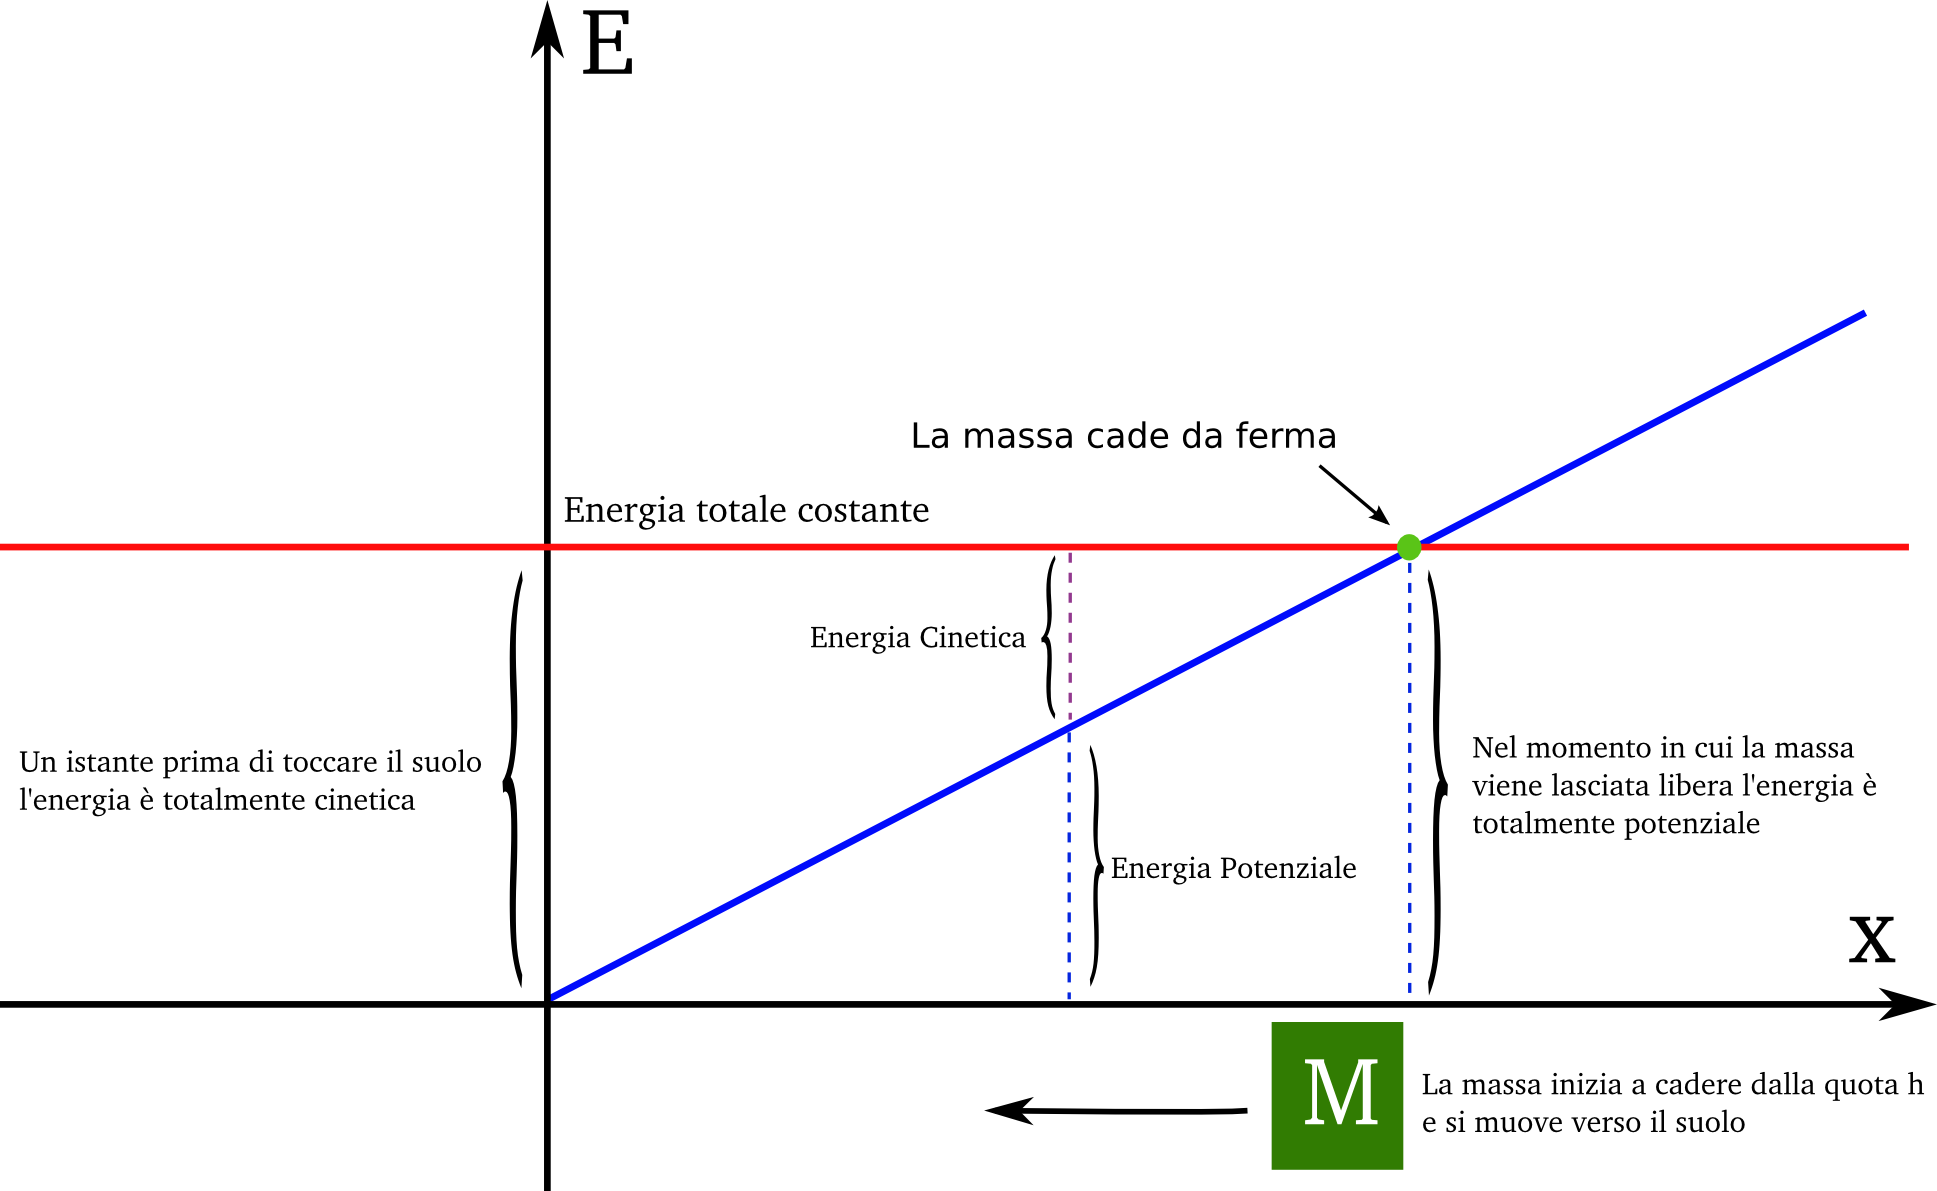
\includegraphics[width=\textwidth]{./immagini/pontenziale_gravitazionale.png}
 % pontenziale_gravitazionale.png: 1937x1191 pixel, 300dpi, 16.40x10.08 cm, bb=0 0 465 286
 \caption{Il corpo di massa $M$ sta cadendo da fermo dalla quota $x=h$ verso il suolo. La retta orizzontale rappresenta l'energia meccanica totale costante del sistema, la retta passante per l'origine l'energia potenziale alla quota $x$}\label{fig:potenziale2}
\end{figure}

Nel caso della massa collegata alla molla, l'energia potenziale non è più lineare ma ha un andamento parabolico. Riportando in un grafico energia-posizione, l'energia potenziale e l'energia totale del sistema figura [\ref{fig:potenziale1}] vediamo che, a differenza del caso gravitazionale, dove una volta giunta al suolo la massa si ferma, se la molla è libera di oscillare attorno al punto di equilibrio \footnote{Il punto di estensione nulla  della molla, quando questa è in quiete} il moto sarà  periodico. Quando la molla si estende fino all'ascissa di intersezione tra il grafico dell'energia totale e quello dell'energia potenziale, la velocità della massa in moto si annulla e l'energia è puramente potenziale, il corpo inverte il suo moto e si sposta fino a raggiungere il punto di inversione simmetrico, dove si ferma e inverte nuovamente il verso del suo moto. In assenza di attrito il moto continuerà fino a che non sarà perturbato da forze esterne.


\begin{figure}[H]
 \centering
 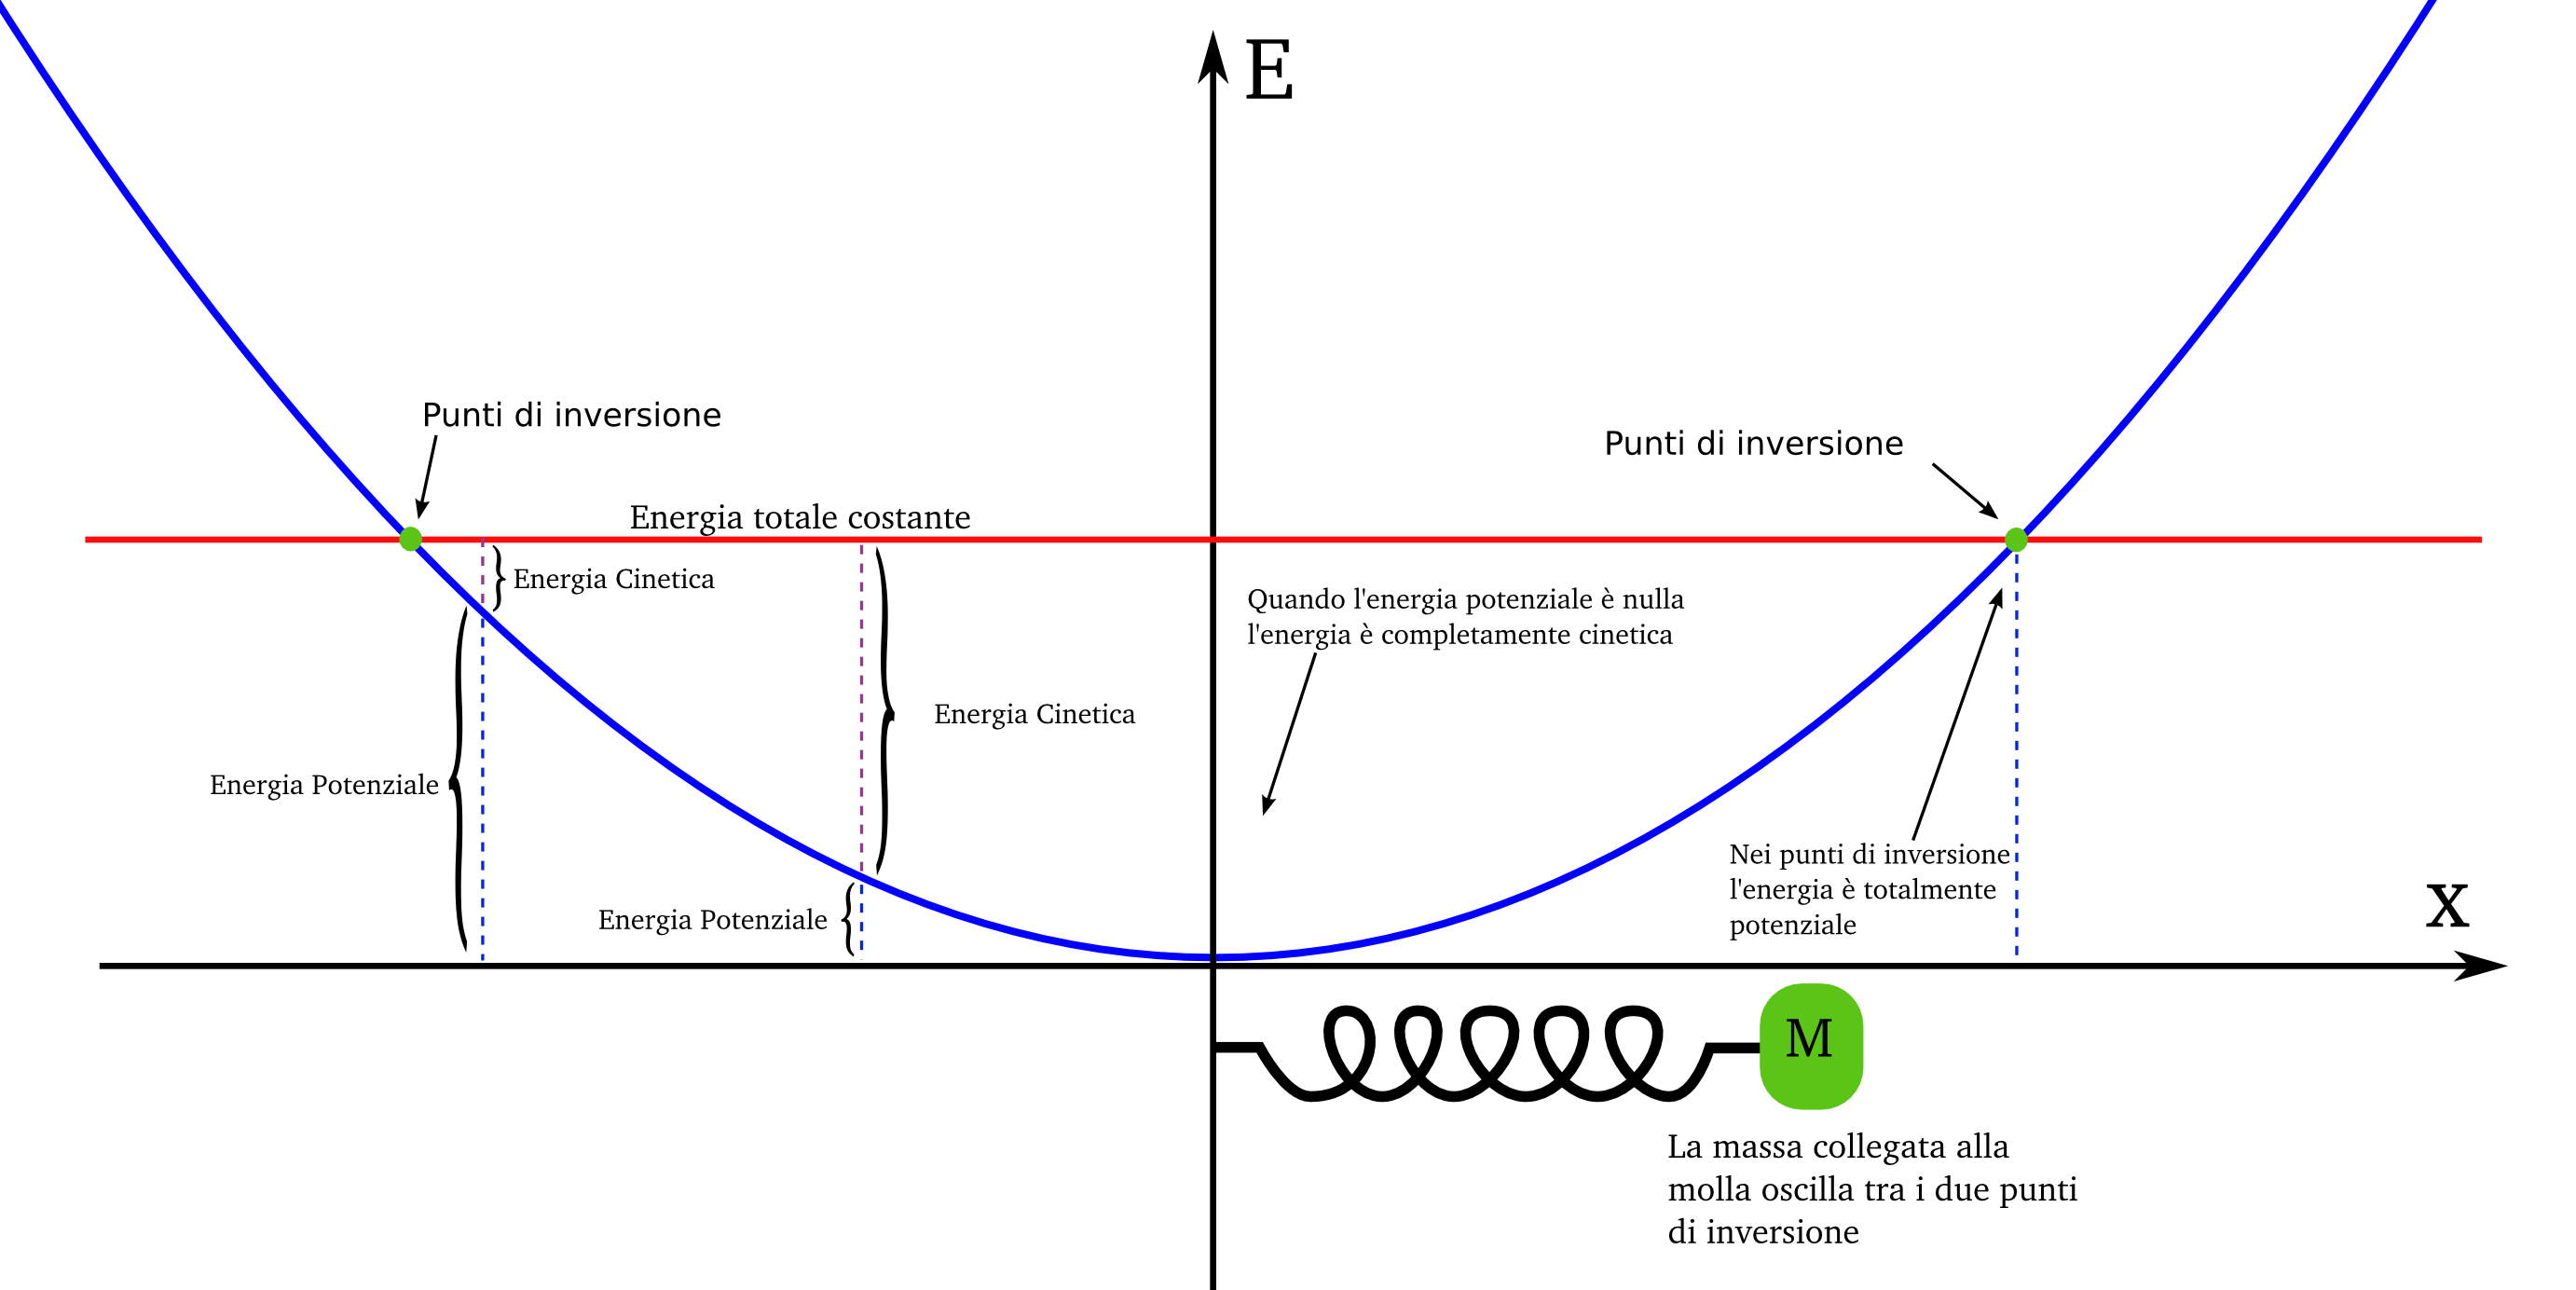
\includegraphics[width=\textwidth]{./immagini/pontenziale_molla.png}
 % pontenziale_molla.png: 2764x1384 pixel, 300dpi, 23.40x11.72 cm, bb=0 0 663 332
 \caption{Il corpo di massa $M$ collegato alla molla oscilla tra le posizioni $x=\overline x$ e $x=-\overline x$}\label{fig:potenziale1}
\end{figure}


\section*{Il moto armonico semplice}

Fino ad ora abbiamo studiato unicamente gli aspetti energetici della forza elastica e non ci siamo interessati del moto di una massa $m$ soggetta alla forza elastica $F=-kx$. Sfortunatamente non disponiamo degli strumenti matematici necessari a risolvere il problema direttamente (come avevamo fatto per il caso della forza costante), è però possibile giungere ad una soluzione soddisfacente del problema, confrontando il moto della massa soggetta alla forza elastica con quello di un oggetto che si muove di moto circolare uniforme.

\begin{figure}[H]
 \centering
 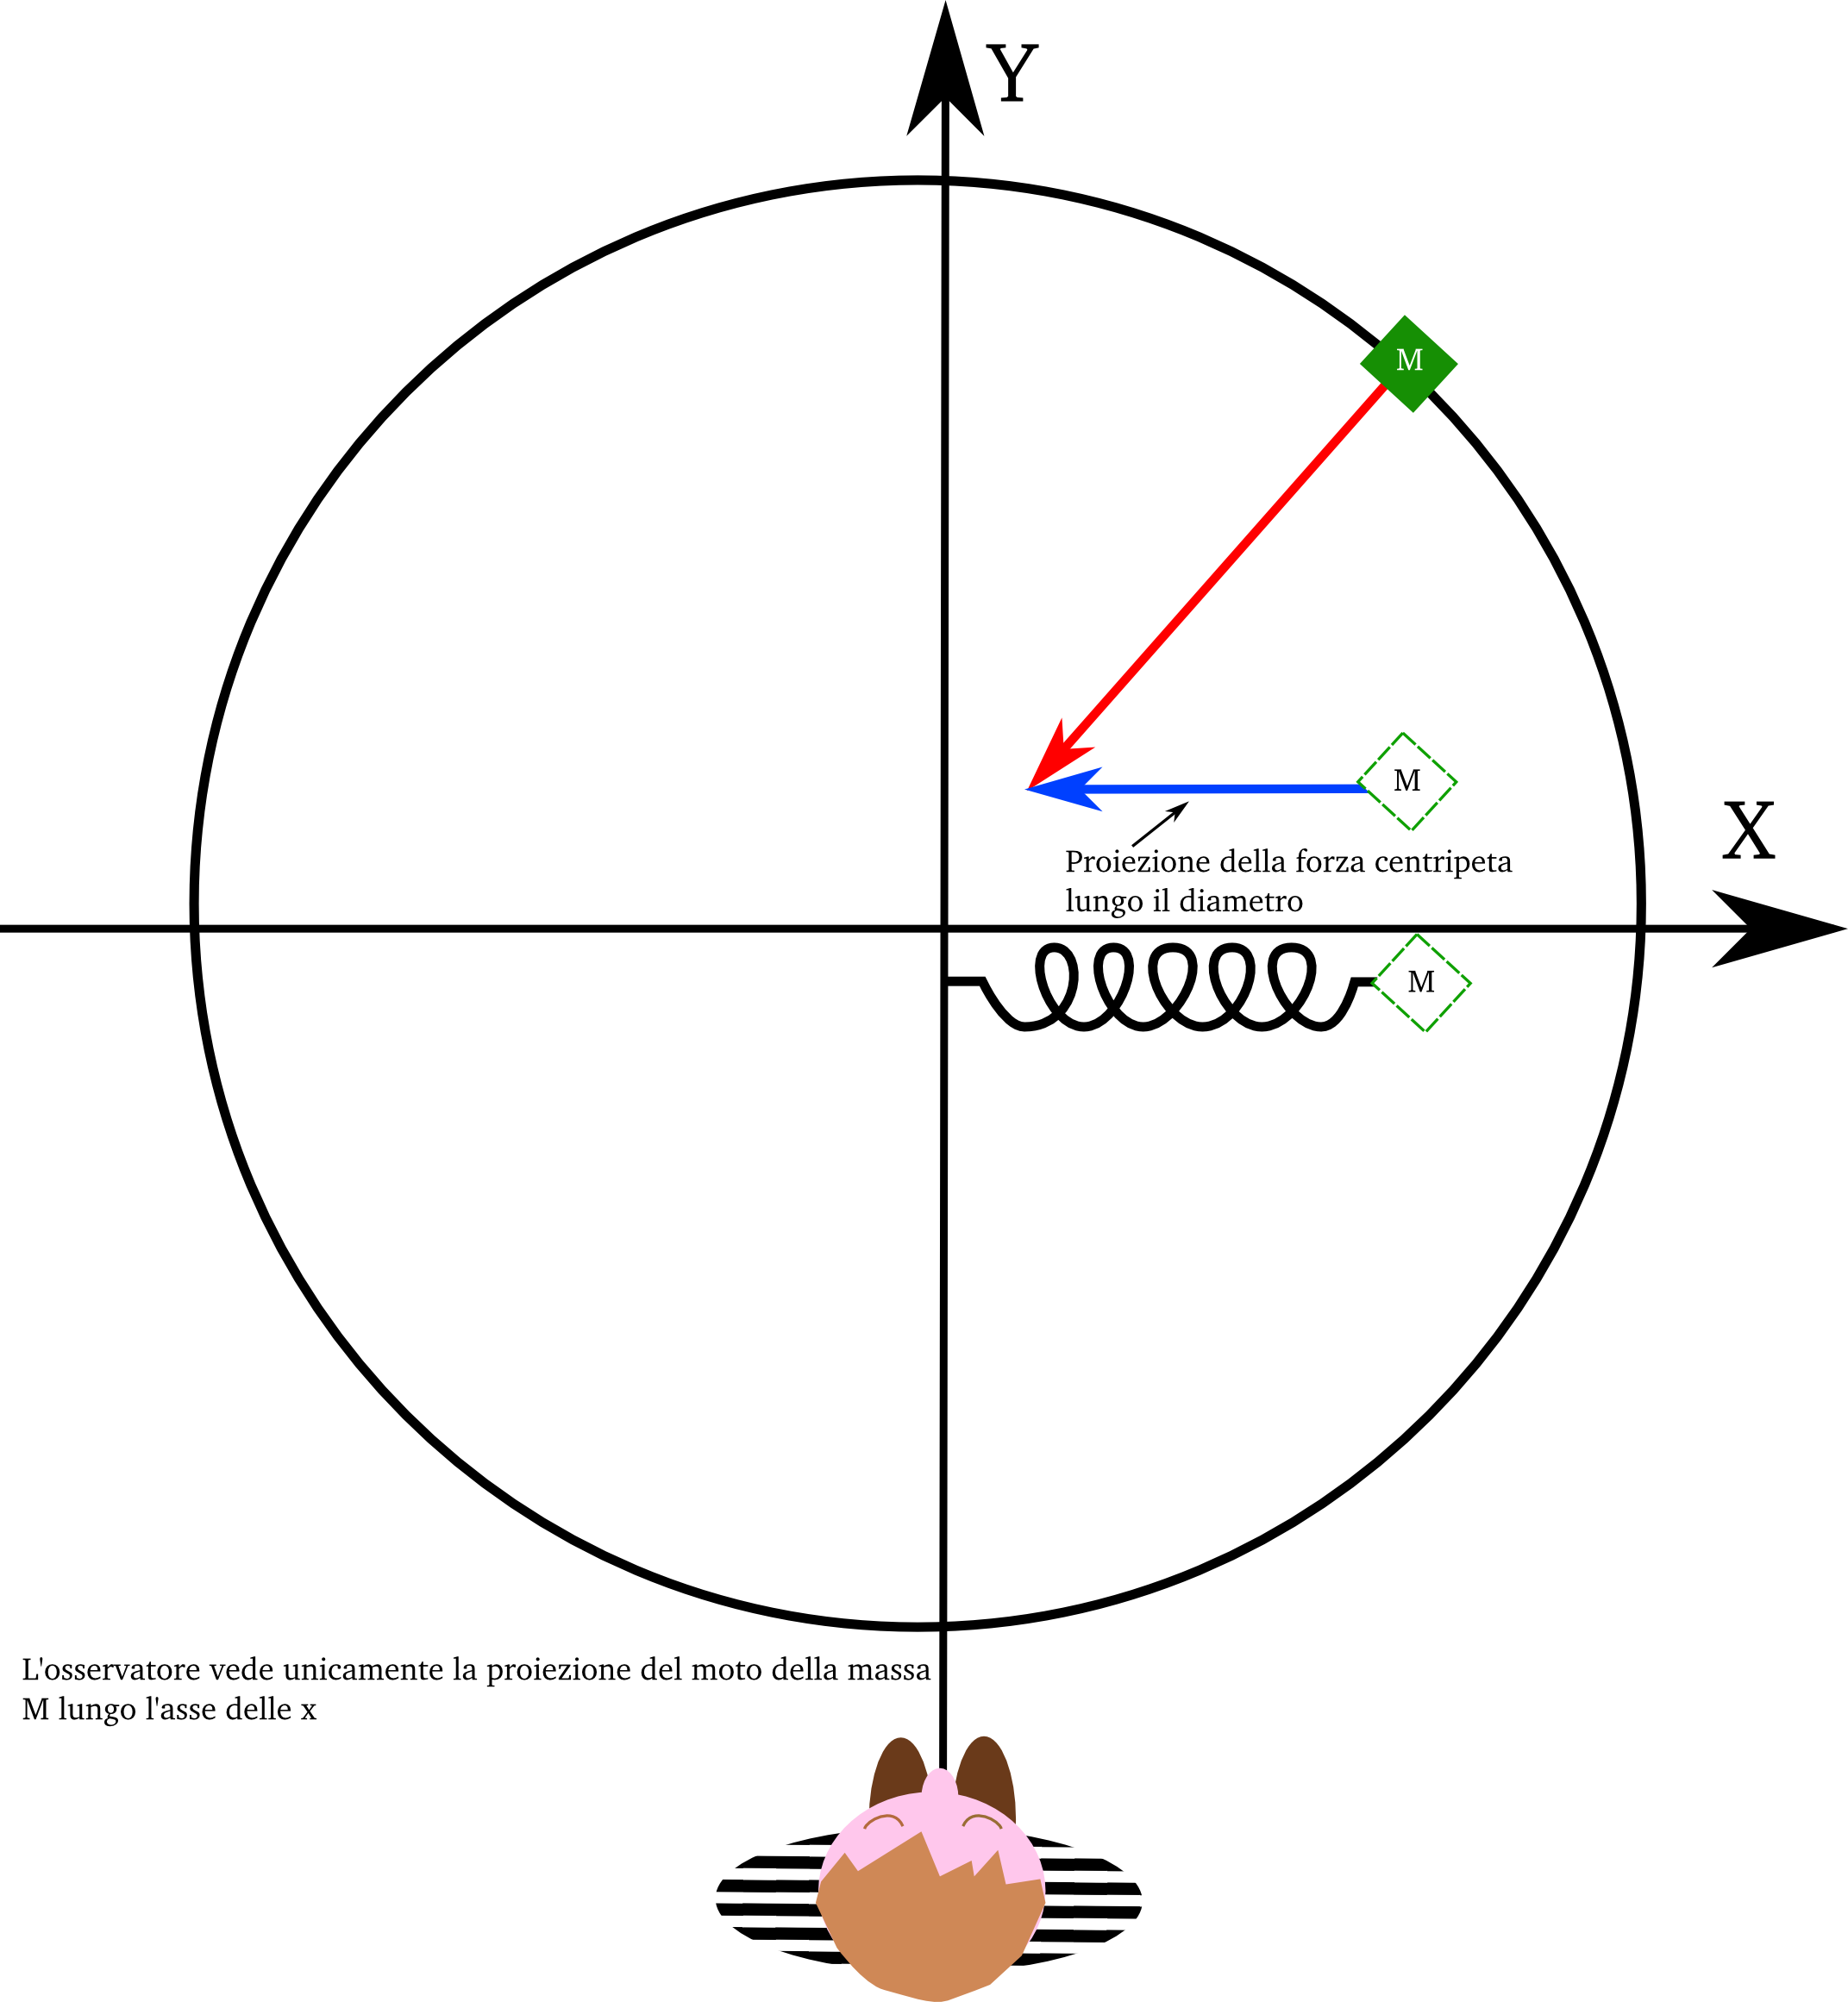
\includegraphics[width=0.8\textwidth]{./immagini/armonico_vista.png}
 % armonico_vista.png: 1944x2142 pixel, 300dpi, 16.46x18.14 cm, bb=0 0 467 514
 \caption{Un osservatore in grado di osservare unicamente la proiezione del moto lungo l'asse delle ascisse non è in grado di distinguere tra il moto di una massa collegata ad una molla, e quello di un oggetto vincolato ad una circonferenza in rotazione uniforme}\label{fig:armonico1}
\end{figure}


Immaginiamo una massa $m$ in moto con velocità angolare costante lungo una circonferenza di raggio $r$ dalla teoria che abbiamo studiato risulta che la componente $x$ della sua accelerazione centripeta è:
\begin{equation}
 a_x=-\omega^2r\cos(\omega t)
\end{equation}
quindi un osservatore disposto in modo da vedere di taglio la rotazione della massa misurerà una forza:
\begin{equation}
 F_x=-m\omega^2r\cos(\omega t)
\end{equation}

ricordando ora che la componente orizzontale del vettore posizione risulta $ x=r\cos\omega t$ possiamo riscrivere la componente $x$ della forza centripeta come:
\begin{equation}
 F_x=-m\omega^2x
\end{equation}
che, dal punto di vista matematico, ha la stessa forma della legge elastica ovvero una costante che moltiplica uno spostamento $x$:
\begin{equation}
 F_e=-kx
\end{equation}
in particolare se scegliamo $\omega$ in modo che sia:
\begin{equation}
 m\omega^2=k
\end{equation}
ovvero:
\begin{equation}\label{omega1}
 \omega=\sqrt{\frac k m}
\end{equation}
la forza elastica e la componente $x$ della forza centripeta risulteranno numericamente identiche, questo ci assicura che i moti risultanti, della massa collegata alla molla e della massa vincolata alla circonferenza rotante sono identici.
Tale importante osservazione ci permette di ricavare la dipendenza temporale dello spostamento della massa vincolata alla molla e la sua velocità, semplicemente riutilizzando le formule ricavate per il moto circolare.
Analizziamo il caso semplice in cui al tempo $t=0$ la massa collegata alla molla si trova alla massima estensione positiva $\overline x$ ovvero $x(0)=\overline x$. Usando la [\ref{omega1}] e la componente $x$ del vettore posizione del moto circolare uniforme, considerando il raggio della circonferenza associata  pari a $\overline x$, possiamo scrivere:
\begin{equation}
 x=\overline x \cos(\omega t)
\end{equation}
e quindi
\begin{equation}
 x=\overline x\cos(\sqrt{\frac k m}t)
\end{equation}
lo stesso discorso si può fare per la velocità, la componente $x$ della velocità della massa collegata alla circonferenza risulta:
\begin{equation}
 v_x=-\omega \overline x\sin(\omega t)
\end{equation}
per cui la velocità della massa collegata alla molla sarà:
\begin{equation}
 v=-\sqrt{\frac k m }\overline x\sin(\sqrt{\frac k m }t)
\end{equation}

\subsection*{Diverse condizioni iniziali}
Nell'esempio precedente abbiamo supposto che la massa fosse lasciata libera al tempo zero con velocità iniziale nulla; se invece decidessimo di impartirle una velocità iniziale diversa da zero cosa succederebbe? Cerchiamo di analizzare il problema utilizzando un esempio. Trattiamo il caso della massa lasciata partire dalla posizione $x=0$ al tempo $t=0$ con velocità iniziale $v_0$. Appare chiaro che l'energia totale della massa collegata  alla molla, nel momento iniziale, è unicamente cinetica possiamo quindi dire che il valore costante dell'energia risulterà:
\begin{equation}
E=\frac 1 2 mv_0^2
\end{equation}
nei punti di inversione la molla sarà istantaneamente ferma per cui l'energia totale risulterà essere totalmente potenziale da cui:
\begin{equation}
 E=\frac 1 2 k \overline x^2
\end{equation}
questo ci permette di determinare il massimo allungamento della molla:
\begin{equation}
 \overline x=\frac{v_0}{\omega}
\end{equation}
Quali saranno le equazioni che descrivono il moto della massa? Notiamo che all'istante $t=0$ la massa deve trovarsi nell'origine quindi l'equazione $x=\overline x\cos(\omega t)$ non sarà più adatta a descrivere il moto\footnote{Infatti il coseno non è mai nullo per argomento nullo} , come possiamo risolvere il problema? Una strada per giungere alla soluzione, senza utilizzare della matematica complessa, è di pensare che il moto in esame non sia altro che un moto iniziato con massa ferma ad una certa distanza dal punto $x=0$ in un tempo \textbf{anteriore} rispetto a quando facciamo partire il cronometro. Immaginate, ad esempio, che qualcuno abbia fatto partire la massa senza dirvi nulla, che la luce del laboratorio sia spenta e che questa venga accesa all'istante del vostro orologio $t=0$  quando la massa si trova a passare per $x=0$ con una certa velocità $v_0$, potremmo quindi pensare che il nostro esperimento con condizioni iniziali diverse non sia altro che il moto semplice già studiato ma iniziato in un tempo $t_0$ anteriore rispetto a quello in cui abbiamo fatto partire il nostro cronometro.
Scriveremo quindi per la posizione $x$ della massa al tempo $t$ la relazione:
\begin{equation}\label{mot_trasl}
 x=\overline x\cos(\omega(t-t_0))
\end{equation}
Quando deve essere iniziato il movimento della massa affinché al tempo $t=0$ questa si trovi nella posizione $x=0$? Per rispondere a questa domanda dobbiamo determinare quando la funzione coseno si annulla. Da quanto avete studiato in matematica sapete che il coseno si annulla in $\frac \pi 2 +k\pi$ quindi per trovare il tempo $t_0$ minimo devo semplicemente uguagliare a $\frac \pi 2 $ l'argomento del coseno nella [\ref{mot_trasl}], ponendo $t=0$:
\begin{equation}
 -\omega t_0=\frac \pi 2
\end{equation}
da cui
\begin{equation}\label{t0}
 t_0=-\frac{\pi}{2\omega}
\end{equation}
Se ricordiamo quanto detto precedentemente, ovvero che $\omega$ rappresenta la pulsazione del moto armonico semplice e che il periodo è pari a:
\begin{equation}
 T=\frac{2\pi}{\omega}
\end{equation}
otteniamo:
\begin{equation}
 t_0=-\frac{T}{4}
\end{equation}
ovvero il moto deve essere iniziato un quarto di periodo prima dell'inizio della misura. Armati di queste informazioni possiamo riscrivere la [\ref{mot_trasl}] sostituendo al posto del tempo iniziale il valore trovato nella [\ref{t0}]:
\begin{equation}
 x=\overline x \cos(\omega t-\omega \frac{\pi}{2\omega})=\overline x \cos(\omega t-\frac \pi 2)
\end{equation}
che ricordando gli archi associati si riduce a :
\begin{equation}
 x=\overline x\sin\omega t
\end{equation}
Durante l'esperienza di laboratorio vedremo cosa succederà in casi diversi quando al tempo $t=0$ la posizione della massa non è nulla ne lo è la sua velocità.

\subsection*{Verifica della conservazione dell'energia}
Grazie alle informazioni ottenute tramite il confronto con il moto circolare uniforme possiamo controllare esplicitamente che la forza elastica è una forza conservativa e che quindi l'energia meccanica della massa collegata alla molla è costante.
\begin{equation}
 E=\frac 1 2 kx^2 +\frac 1 2 mv^2=\frac 1 2 kx^2 +\frac 1 2m \left(-\sqrt{\frac k m }\overline x\sin(\sqrt{\frac k m }t)\right)^2
\end{equation}
svolgendo alcuni calcoli otteniamo:
\begin{equation}\label{cons_mol1}
 E=\frac 1 2 kx^2+\frac 1 2  k \overline x^2\left(\sin( \sqrt{\frac k m}t)\right)^2
\end{equation}

applicando alla [\ref{cons_mol1}] la relazione goniometrica fondamentale $\sin^2 \alpha+\cos^2\alpha=1$ otteniamo:
\begin{equation}
 E=\frac 1 2 kx^2+\frac1 2 k\overline x^2-\frac 1 2 kx^2
\end{equation}
dove si è usato il fatto che $\left(\overline x \cos( \sqrt{\frac k m}t)\right)^2=x^2$. Per cui l'energia totale del sistema è pari a\footnote{Nel caso in cui la massa venga lasciata da ferma al tempo $t=0$ nella posizione $x(0)=\overline x$}:
                                                                                                                                     \begin{equation}                                                                                                                                   E=\frac 1 2 k\overline x^2                                                                                                                                    \end{equation}
Come avevamo precedentemente anticipato l'energia totale della massa collegata alla molla è una \emph{costante del moto}.





 

\end{document}
